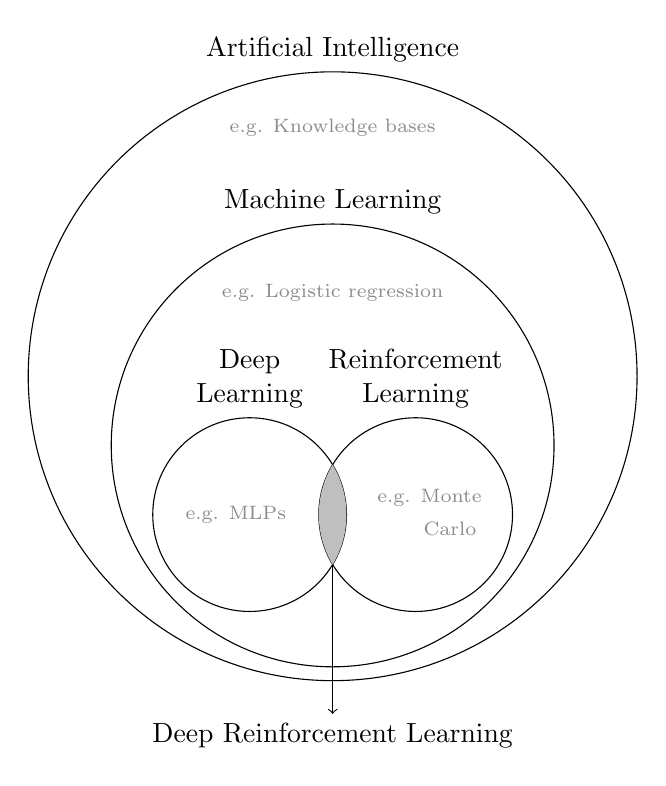
\begin{tikzpicture}

    % Circle with label
    \node[draw,
        circle,
        minimum size =22em,
        label=Artificial Intelligence] (ai_circ) at (0,0){};

    % Circle with label
    \node[draw,
        circle,
        minimum size =16em,
        label=Machine Learning] (ml_circ) at (0,-2.5em){};

    % Circle with label
    \node[draw,
        circle,
        minimum size =7em,
        label={[align=center]Deep \\ Learning}] (dl_circ) at (-3em,-5em){};

    \node[draw,
        circle,
        minimum size =7em,
        label= {[align=center]Reinforcement \\ Learning}] (rl_circ) at (3em,-5em){};

    \node[] (dlrl) at (0em,-13em){Deep Reinforcement Learning};
    \draw[<-] (dlrl.north) -- (0em, -4em);

    % Intersection
    \begin{scope}
        \clip (-3em,-5em) circle(3.5em);
        \clip (3em,-5em) circle(3.5em);
        \fill[gray!50](3em,-5em) circle(3.5em);
    \end{scope}

    \node[anchor=center, text=gray!90] at (0em, 9em) {\scriptsize e.g. Knowledge bases};
    \node[anchor=center, text=gray!90] at (0em, 3em) {\scriptsize e.g. Logistic regression};
    \node[anchor=center, text=gray!90] at (-3.5em, -5em) {\scriptsize e.g. MLPs};
    \node[anchor=center,align=center, text=gray!90] at (3.5em, -5em) {\scriptsize e.g. Monte \\ \scriptsize \phantom{e.g.} Carlo};


\end{tikzpicture}